\chapter{Задание}
Цель работы: построение доверительных интервалов для математического ожидания и дисперсии нормальной случайной величины.
\section{Содержание работы}
\begin{enumerate}
	\item Для выборки объема n из нормальной генеральной совокупности X реализовать в виде программы на ЭВМ
	\begin{enumerate}
		\item вычисление точечных оценок $\hat{\mu}(\vec{x}_n)$ и $S^2(\vec{x}_n)$
		MX и дисперсии DX; соответственно;
		\item вычисление нижней и верхней границ $\underline{{\mu}}(\vec{x}_n)$, $\overline{{\mu}}(\vec{x}_n)$ для \newline $\gamma$-доверительного интервала для
		математического ожидания MX;
		\item вычисление нижней и верхней границ 
		$\underline{\sigma^2}(\vec{x}_n)$, 
		$\overline{\sigma^2}(\vec{x}_n)$ для \newline $\gamma$-доверительного интервала для
		дисперсии DX;
	\end{enumerate}
	\item Вычислить $\hat{\mu}(\vec{x}_n)$ и $S^2(\vec{x}_n)$ для выборки из индивидуального варианта;
	\item Для заданного пользователем уровня доверия $\gamma$ и N – объема выборки из индивидуального варианта:
	\begin{enumerate}
		\item на координатной плоскости $Oyn$ построить прямую $y=\hat{\mu}(\vec{x}_N)$, также графики функций $y=\hat{\mu}(\vec{x}_n)$
		$y=\underline{{\mu}}(\vec{x}_n)$, $y=\overline{{\mu}}(\vec{x}_n)$,  как функций объема n выборки, где n изменяется от 1 до N;
		\item на другой координатной плоскости $Ozn$ построить прямую $z = S^2(\vec{x}_N)$, также графики
		функций $z = S^2(\vec{x}_n)$, $z = \underline{\sigma^2}(\vec{x}_n)$
		и $z = \overline{\sigma^2}(\vec{x}_n)$ как функций объема n выборки, где n
		изменяется от 1 до N.
	\end{enumerate}
\end{enumerate}

\chapter{Теоретическая часть}

Пусть $\vec{x} = (x_1, \dots, x_n)$ --- реализация случайной выборки из генеральной совокупности случайно величины X, закон распределения которой известен с точностью до параметра $\theta$.

$\gamma$--доверительным интервалом для параметра $\theta$ называется интервал $(\underline{\theta}, \overline{\theta})$ для которого справедливо $P(\underline{\theta} \leq \theta \leq \overline{\theta}) = \gamma$.

В работе использовались следующие формулы для вычисления величин:
\begin{gather}
	\label{mu}
	\overline{x} = \frac{1}{n}\sum_{i = 1}^{N}~x_i;\\
	\label{s}
	S^2 = \frac{1}{n - 1}\sum_{i = 1}^{N}~(x_i - \overline{x})^2;\\
	\label{mu_low}
	\underline{\mu}(\vec{x}_n) = \overline{x} - \frac{S}{\sqrt{n}}t_{1-\alpha}(n-1)\\
	\label{mu_high}
	\overline{\mu}(\vec{x}_n) = \overline{x} + \frac{S}{\sqrt{n}}t_{1-\alpha}(n-1)\\
	\label{sigma_low}
	\underline{\sigma}(\vec{x}_n) = \frac{S^2(n-1)}{\chi^2_{1-\alpha}(n-1)}\\
	\label{sigma_high}
	\overline{\sigma}(\vec{x}_n) = \frac{S^2(n-1)}{\chi^2_\alpha(n-1)}
\end{gather}

где (\ref{mu}) --- точечная оценка математического ожидания, (\ref{s}) --- точечная оценка дисперсии, (\ref{mu_low}) --- нижняя граница $\gamma$--доверительного интервала для математического ожидания, (\ref{mu_high}) --- верхняя граница $\gamma$--доверительного интервала для математического ожидания, (\ref{sigma_low}) --- нижняя граница $\gamma$--доверительного интервала для дисперсии, верхняя граница $\gamma$--доверительного интервала для дисперсии, $t_{\alpha}(n-1)$ --- квантиль уровня $(1 - \alpha)$ распределения Стьюдента c (n - 1) степенями свободы, $\chi^2_{\alpha}(n-1)$ --- квантиль уровня $\alpha$ распределения $\chi^2$.

\chapter{Практическая часть}

Значения параметров для выборки из индивидуального варианта №10:

$\hat{\mu}(\overrightarrow{x}_n)= 1.836417$;

$S^2(\overrightarrow{x}_n)= 1.152669$.

Результаты построения графиков функций:
\begin{figure}[h]
	\centering{
		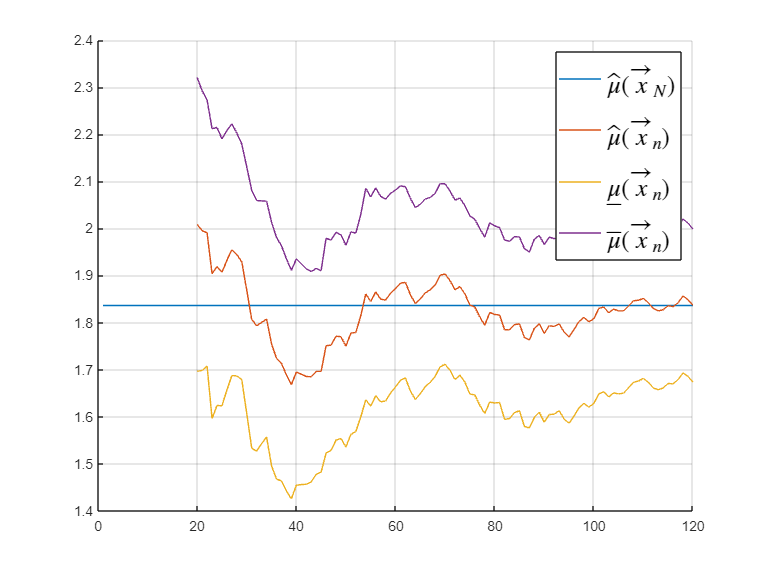
\includegraphics[scale=0.8]{./img/1}
		\caption{Графики прямой $y = \hat{\mu}(\vec{x}_N)$, а также функций $y = \hat{\mu}(\vec{x}_n)$
			$y=\underline{{\mu}}(\vec{x}_n)$, $y=\overline{{\mu}}(\vec{x}_n)$,  как функций объема n выборки, где n изменяется от 1 до N}
		\label{image:1}
	}
\end{figure}

\clearpage

\begin{figure}[h]
	\centering{
		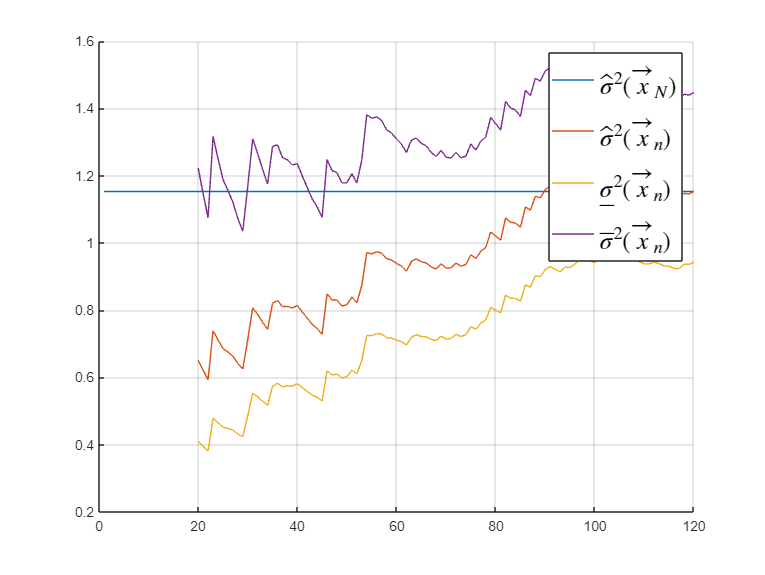
\includegraphics[scale=0.8]{./img/2}
		\caption{Графики прямой $z = S^2(\vec{x}_N)$, также
			функций $z = S^2(\vec{x}_n)$, $z = \underline{\sigma^2}(\vec{x}_n)$
			и $z = \overline{\sigma^2}(\vec{x}_n)$ как функций объема n выборки, где n
			изменяется от 1 до N}
		\label{image:2}
	}
\end{figure}